% Options for packages loaded elsewhere
\PassOptionsToPackage{unicode}{hyperref}
\PassOptionsToPackage{hyphens}{url}
%
\documentclass[
]{book}
\usepackage{amsmath,amssymb}
\usepackage{lmodern}
\usepackage{ifxetex,ifluatex}
\ifnum 0\ifxetex 1\fi\ifluatex 1\fi=0 % if pdftex
  \usepackage[T1]{fontenc}
  \usepackage[utf8]{inputenc}
  \usepackage{textcomp} % provide euro and other symbols
\else % if luatex or xetex
  \usepackage{unicode-math}
  \defaultfontfeatures{Scale=MatchLowercase}
  \defaultfontfeatures[\rmfamily]{Ligatures=TeX,Scale=1}
\fi
% Use upquote if available, for straight quotes in verbatim environments
\IfFileExists{upquote.sty}{\usepackage{upquote}}{}
\IfFileExists{microtype.sty}{% use microtype if available
  \usepackage[]{microtype}
  \UseMicrotypeSet[protrusion]{basicmath} % disable protrusion for tt fonts
}{}
\makeatletter
\@ifundefined{KOMAClassName}{% if non-KOMA class
  \IfFileExists{parskip.sty}{%
    \usepackage{parskip}
  }{% else
    \setlength{\parindent}{0pt}
    \setlength{\parskip}{6pt plus 2pt minus 1pt}}
}{% if KOMA class
  \KOMAoptions{parskip=half}}
\makeatother
\usepackage{xcolor}
\IfFileExists{xurl.sty}{\usepackage{xurl}}{} % add URL line breaks if available
\IfFileExists{bookmark.sty}{\usepackage{bookmark}}{\usepackage{hyperref}}
\hypersetup{
  pdftitle={Supplementary Materials for Gene Co-expression Network Estimation for Spatial Transcriptomics},
  pdfauthor={Satwik Acharyya, Xiang Zhou, Veera Baladandayuthapani},
  hidelinks,
  pdfcreator={LaTeX via pandoc}}
\urlstyle{same} % disable monospaced font for URLs
\usepackage{color}
\usepackage{fancyvrb}
\newcommand{\VerbBar}{|}
\newcommand{\VERB}{\Verb[commandchars=\\\{\}]}
\DefineVerbatimEnvironment{Highlighting}{Verbatim}{commandchars=\\\{\}}
% Add ',fontsize=\small' for more characters per line
\usepackage{framed}
\definecolor{shadecolor}{RGB}{248,248,248}
\newenvironment{Shaded}{\begin{snugshade}}{\end{snugshade}}
\newcommand{\AlertTok}[1]{\textcolor[rgb]{0.94,0.16,0.16}{#1}}
\newcommand{\AnnotationTok}[1]{\textcolor[rgb]{0.56,0.35,0.01}{\textbf{\textit{#1}}}}
\newcommand{\AttributeTok}[1]{\textcolor[rgb]{0.77,0.63,0.00}{#1}}
\newcommand{\BaseNTok}[1]{\textcolor[rgb]{0.00,0.00,0.81}{#1}}
\newcommand{\BuiltInTok}[1]{#1}
\newcommand{\CharTok}[1]{\textcolor[rgb]{0.31,0.60,0.02}{#1}}
\newcommand{\CommentTok}[1]{\textcolor[rgb]{0.56,0.35,0.01}{\textit{#1}}}
\newcommand{\CommentVarTok}[1]{\textcolor[rgb]{0.56,0.35,0.01}{\textbf{\textit{#1}}}}
\newcommand{\ConstantTok}[1]{\textcolor[rgb]{0.00,0.00,0.00}{#1}}
\newcommand{\ControlFlowTok}[1]{\textcolor[rgb]{0.13,0.29,0.53}{\textbf{#1}}}
\newcommand{\DataTypeTok}[1]{\textcolor[rgb]{0.13,0.29,0.53}{#1}}
\newcommand{\DecValTok}[1]{\textcolor[rgb]{0.00,0.00,0.81}{#1}}
\newcommand{\DocumentationTok}[1]{\textcolor[rgb]{0.56,0.35,0.01}{\textbf{\textit{#1}}}}
\newcommand{\ErrorTok}[1]{\textcolor[rgb]{0.64,0.00,0.00}{\textbf{#1}}}
\newcommand{\ExtensionTok}[1]{#1}
\newcommand{\FloatTok}[1]{\textcolor[rgb]{0.00,0.00,0.81}{#1}}
\newcommand{\FunctionTok}[1]{\textcolor[rgb]{0.00,0.00,0.00}{#1}}
\newcommand{\ImportTok}[1]{#1}
\newcommand{\InformationTok}[1]{\textcolor[rgb]{0.56,0.35,0.01}{\textbf{\textit{#1}}}}
\newcommand{\KeywordTok}[1]{\textcolor[rgb]{0.13,0.29,0.53}{\textbf{#1}}}
\newcommand{\NormalTok}[1]{#1}
\newcommand{\OperatorTok}[1]{\textcolor[rgb]{0.81,0.36,0.00}{\textbf{#1}}}
\newcommand{\OtherTok}[1]{\textcolor[rgb]{0.56,0.35,0.01}{#1}}
\newcommand{\PreprocessorTok}[1]{\textcolor[rgb]{0.56,0.35,0.01}{\textit{#1}}}
\newcommand{\RegionMarkerTok}[1]{#1}
\newcommand{\SpecialCharTok}[1]{\textcolor[rgb]{0.00,0.00,0.00}{#1}}
\newcommand{\SpecialStringTok}[1]{\textcolor[rgb]{0.31,0.60,0.02}{#1}}
\newcommand{\StringTok}[1]{\textcolor[rgb]{0.31,0.60,0.02}{#1}}
\newcommand{\VariableTok}[1]{\textcolor[rgb]{0.00,0.00,0.00}{#1}}
\newcommand{\VerbatimStringTok}[1]{\textcolor[rgb]{0.31,0.60,0.02}{#1}}
\newcommand{\WarningTok}[1]{\textcolor[rgb]{0.56,0.35,0.01}{\textbf{\textit{#1}}}}
\usepackage{longtable,booktabs,array}
\usepackage{calc} % for calculating minipage widths
% Correct order of tables after \paragraph or \subparagraph
\usepackage{etoolbox}
\makeatletter
\patchcmd\longtable{\par}{\if@noskipsec\mbox{}\fi\par}{}{}
\makeatother
% Allow footnotes in longtable head/foot
\IfFileExists{footnotehyper.sty}{\usepackage{footnotehyper}}{\usepackage{footnote}}
\makesavenoteenv{longtable}
\usepackage{graphicx}
\makeatletter
\def\maxwidth{\ifdim\Gin@nat@width>\linewidth\linewidth\else\Gin@nat@width\fi}
\def\maxheight{\ifdim\Gin@nat@height>\textheight\textheight\else\Gin@nat@height\fi}
\makeatother
% Scale images if necessary, so that they will not overflow the page
% margins by default, and it is still possible to overwrite the defaults
% using explicit options in \includegraphics[width, height, ...]{}
\setkeys{Gin}{width=\maxwidth,height=\maxheight,keepaspectratio}
% Set default figure placement to htbp
\makeatletter
\def\fps@figure{htbp}
\makeatother
\setlength{\emergencystretch}{3em} % prevent overfull lines
\providecommand{\tightlist}{%
  \setlength{\itemsep}{0pt}\setlength{\parskip}{0pt}}
\setcounter{secnumdepth}{5}
\usepackage{booktabs}
\usepackage{amsthm}
\makeatletter
\def\thm@space@setup{%
  \thm@preskip=8pt plus 2pt minus 4pt
  \thm@postskip=\thm@preskip
}
\makeatother
\usepackage{booktabs}

\def\T{{ \mathrm{\scriptscriptstyle T} }}
\def\tr{{\rm tr\,}}
\ifluatex
  \usepackage{selnolig}  % disable illegal ligatures
\fi
\usepackage[]{natbib}
\bibliographystyle{apalike}

\title{Supplementary Materials for Gene Co-expression Network Estimation for Spatial Transcriptomics}
\author{Satwik Acharyya, Xiang Zhou, Veera Baladandayuthapani}
\date{2021-12-23}

\begin{document}
\maketitle

{
\setcounter{tocdepth}{1}
\tableofcontents
}
\hypertarget{appendix-supplementary-materials}{%
\appendix}


\hypertarget{introduction}{%
\chapter*{Introduction}\label{introduction}}
\addcontentsline{toc}{chapter}{Introduction}

The spatial transcriptomics method depicts the positioning of a single cell on a spatially structured tissue. Knowledge about gene expressions and the spatial distribution of mRNA allows us to uncover cellular and subcellular heterogeneity in tissues, tumors, and immune cells. Spatial transcriptomics provides a unique opportunity to decipher both the cellular and subcellular architecture in both tissues and individual cells along with detection of gene co-expression patterns at both levels. These approaches are very insightful to study disease propagation in the field of embryology, oncology, and histology. The SpaceX method is a statistical tool to quantify spatially varying gene co-expression patterns in a tissue consists of different cell type based or sptailly contiguous clusters.

This is a supplementary file of the paper named SpaceX: Gene Co-expression Network Estimation in Spatial Transcriptomics. The sectional contents of the supplementary file is mentioned below.

\begin{enumerate}
\def\labelenumi{\arabic{enumi}.}
\tightlist
\item
  We start with a detailed description of the methodology in section \ref{method}.
\item
  In section \ref{simulation}, further details of simulation study have been discussed.
\item
  Eploratory analysis and more findings of real data analysis have been laid out in section \ref{realdata}.
\item
  Finally, we discuss the detailed steps for implementation of the SpaceX package in section \ref{ImplementSpaceX}.
\end{enumerate}

\hypertarget{method}{%
\chapter{Methodology}\label{method}}

In this section, we provide a detailed discussion of the estimation procedure for the SpaceX model equation 1 in section 2.1 of the paper. A full-scale MCMC will be computationally expensive on a complex hierarchical model. For computational advantage, we decompose the model into two parts (I) sPMM: spatial Poisson mixed model \citep{sun2017differential} and (II) MSFA: Multi-study factor analysis model \citep{de2018bayesian}. We enable this model decomposition through a standard Gaussian random variable.

\hypertarget{poisson-mixed-model}{%
\section{Poisson Mixed Model}\label{poisson-mixed-model}}

We can break the SpaceX model and write the spatial Poisson mixed model as

\begin{align}
\begin{split}
& \text{log}({\boldsymbol \lambda}^{c}_{g}) = {{\bf X}^{c}}^{T} {\boldsymbol \beta}^{c}_{g} + {\bf s}^{c} + {\bf z}^{c}_{g}, \\
& {\boldsymbol \lambda}^{c}_{g} = ( \lambda^{c}_{1g}, \dots , \lambda^{c}_{N_{c}g} )^{T}, \\
&{\bf s}^{c} = ( s^{c}_{1}, \dots , s^{c}_{N_{c}} )^{T} \sim \text{MVN}(0, \sigma_{1}^{2}\Omega^{c}(s)), \\
&{\bf z}^{c}_{g} = (z^{1}_{1g}, \dots , z^{c}_{N_{c}g})^{T} \sim \text{MVN}(0, \sigma_{2}^{2} I_{N_{c} \times N_{c} }).
\end{split}
\label{eq:PMM-supp}
\end{align}

Here \(\Omega^{c}(s_{1}, s_{2}) = \text{exp} (- \mid \mid s_{1} - s_{2} \mid \mid^{2} / 2 \rho^{2}_{c} ),\) \(c = 1, \dots, C\). We estimate the length scale parameter of spatial kernel \(\rho_{c}\) based on the steps discussed in section 1 of supplementary information in \citet{sun2017differential}. Here \(Z^{c}_{g}\) captures the cluster specific latent gene expressions and a multi-variate hierarchical modeling of \(Z^{c}_{g}(s_{i})\) will help us to identify the gene co-expression network.

\hypertarget{multi-study-factor-model-msfa}{%
\section{Multi-Study Factor Model (MSFA)}\label{multi-study-factor-model-msfa}}

The 2nd stage of the modeling framework is multi-study factor analysis \citep{de2018bayesian} which is provided as follows
\begin{align}
\begin{split}
& \hat{\bf z}^{c}_{i} = \boldsymbol \Phi {\bf f}_{i} + \boldsymbol \Psi^{c} {\bf d}^{c}_{i} + {\bf e}^{c}_{i}, \\
& {\bf f}_{i} \sim N_{K}(0, {\bf I}_{K}), \hspace{0.5cm} {\bf d}^{c}_{i} \sim N_{K_{c}}(0,{\bf I}_{K_{c}}),\\
& {\bf e}^{c}_{i} \sim N_{G}(0,\boldsymbol \Xi_{c}), \hspace{0.5cm} \boldsymbol \Xi_{c} = \text{diag}(\xi^{c}_{1}, \dots, \xi^{c}_{G} ).
\end{split}
\label{eq:MSFA-supp}
\end{align}
The marginal distribution of \(\hat{\bf z}^{c}_{i}\) is a multivariate normal distribution with mean \(0\) and covariance matrix \(\Sigma_{c}\) s.t.
\begin{align}
\Sigma_{c} = \Phi \Phi^{T} + \Psi^{c} {\Psi^{c}}^{T} + \Xi_{c} = \Sigma_{\Phi} + \Sigma_{\Psi^{c}} + \Xi_{c}
\label{eq:sigma-decomposition}
\end{align}
\(\Sigma_{\Phi} = \Phi \Phi^{T}\) and \(\Sigma_{\Psi^{c}} = \Psi^{c} {\Psi^{c}}^{T}\) are covariance of shared and cluster specific factors respectively. The decomposition of \(\Sigma_{c}\) in \eqref{eq:sigma-decomposition} is not a unique since we can set \(\Phi^{*} = \Phi Q\) and \({\Psi^{*}}^{c} = \Psi^{c} Q_{c}\) where \(Q\) and \(Q_{c}\) are square orthonormal matrices. This will also lead to the same decomposition \(\Sigma^{c} = \Phi^{*} {\Phi^{*}}^{T} + {\Psi^{*}}^{c} {{\Psi^{*}}^{c}}^{T} = \Phi \Phi^{T} + \Psi_{c} \Psi_{c}^{T}\). To overcome the indeterminacy through orthonormal matrices, the factor loading matrices are restricted to be lower triangular matrices \citep{geweke1996measuring, lopes2004bayesian}.

\hypertarget{multiplicative-gamma-shrinkage-prior}{%
\section{Multiplicative gamma shrinkage prior}\label{multiplicative-gamma-shrinkage-prior}}

We follow the same steps from \citet{de2018bayesian} and place multiplicative gamma shrinkage prior \citep{bhattacharya2011sparse} prior on the shared and cluster specific loading matrices i.e.~\(\Phi\) and \(\Psi_{c}\) \(c=1,\dots,C\). The shared and cluster specific latent factors (\(K\) and \(K_{c}\) respectively) are selected following methodology described in section 3.3 of \citet{de2018bayesian}. The multiplicative gamma prior on elements of shared covariance matrices are provided as follows
\begin{equation}
\begin{split}
& \phi_{gk} \mid \delta_{gk}, \eta_{k} \sim N(0, \delta_{gk}^{-1} \eta_{k}^{-1}), \hspace{0.5cm} g = 1, \dots , G, \hspace{0.25cm} k = 1, \dots, \infty, \\
& \delta_{gk} \sim \Gamma(\frac{\nu}{2}, \frac{\nu}{2}) \hspace{0.5cm}  \eta_{k} = \prod_{j=1}^{k} \zeta_{j} \hspace{0.5cm} \zeta_{1} \sim \Gamma(a_{1},1) \hspace{0.5cm}  \zeta_{j} \sim \Gamma(a_{2},1), \hspace{0.2cm} j \ge 2. 
\end{split}
\end{equation}
Here \(\delta_{gk}\) is the local shrinkage parameter for \(G\) column elements of \(k\)th column and \(\eta_{k}\) is the global shrinkage parameter where \(\zeta_{j}\) \((j=1,2. \dots)\) are independent. We repeat the same process to posit prior on the elements of cluster-specific loading matrices

\begin{equation}
\begin{split}
& \psi^{c}_{gk_{c}} \mid \delta^{c}_{gk_{c}}, \eta^{c}_{k_{c}} \sim N(0, {\delta^{c^{-1}}_{gk_{c}}} {\eta^{c^{-1}}_{k_{c}}}), \hspace{0.5cm} g = 1, \dots , G, \hspace{0.2cm} k_{c} = 1, \dots, \infty \hspace{0.2cm} \text{and} \hspace{0.2cm} c = 1, \dots , C,\\
& \delta^{c}_{gk_{c}} \sim \Gamma(\frac{\nu^{c}}{2}, \frac{\nu^{c}}{2}) \hspace{0.5cm}  \eta^{c}_{k_{c}} = \prod_{j=1}^{k_{c}} \zeta^{c}_{j} \hspace{0.5cm} \zeta^{c}_{1} \sim \Gamma(a^{c}_{1},1) \hspace{0.5cm}  \zeta^{c}_{j} \sim \Gamma(a^{c}_{2},1), \hspace{0.2cm} j \ge 2.
\end{split}
\end{equation}
Here \(\delta^{c}_{gk_{c}}\) \(\eta^{c}_{k_{c}}\) are local and global parameters respectively and \(\zeta_{j}^{c}\) \((c=1,2, \dots C)\) are independent of each other. We determine \(K\) and \(K_{c}\) following methodology described in section 3.3 of \citet{de2018bayesian}.

\hypertarget{simulation}{%
\chapter{Simulation Study}\label{simulation}}

\hypertarget{induced-correlation-study}{%
\section{Induced Correlation Study}\label{induced-correlation-study}}

In this section, we provide more details about the simulation study. First we consider \(3\) different values of \(\rho\) \((0.1,0.15,0.2)\) and make a induced correlation plot by using the squared exponential spatial kernel. The plots are generented for all cell types and cell type specific cases. The vertical line denotes the value of induced correlation at the distance \(0.01\). For example the induced spatial correlations for all cell types (first figure of \ref{fig:induceCORR}) w.r.t. \(0.01\) distance are \(0.88\), \(0.80\), \(0.61\) for \(\text S_{\text High}\) (\(\rho = 0.2\)), \(\text S_{\text Med}\) (\(\rho = 0.15\)), \(\text S_{\text Low}\) (\(\rho = 0.1\)) methods respectively.

\begin{figure}

{\centering 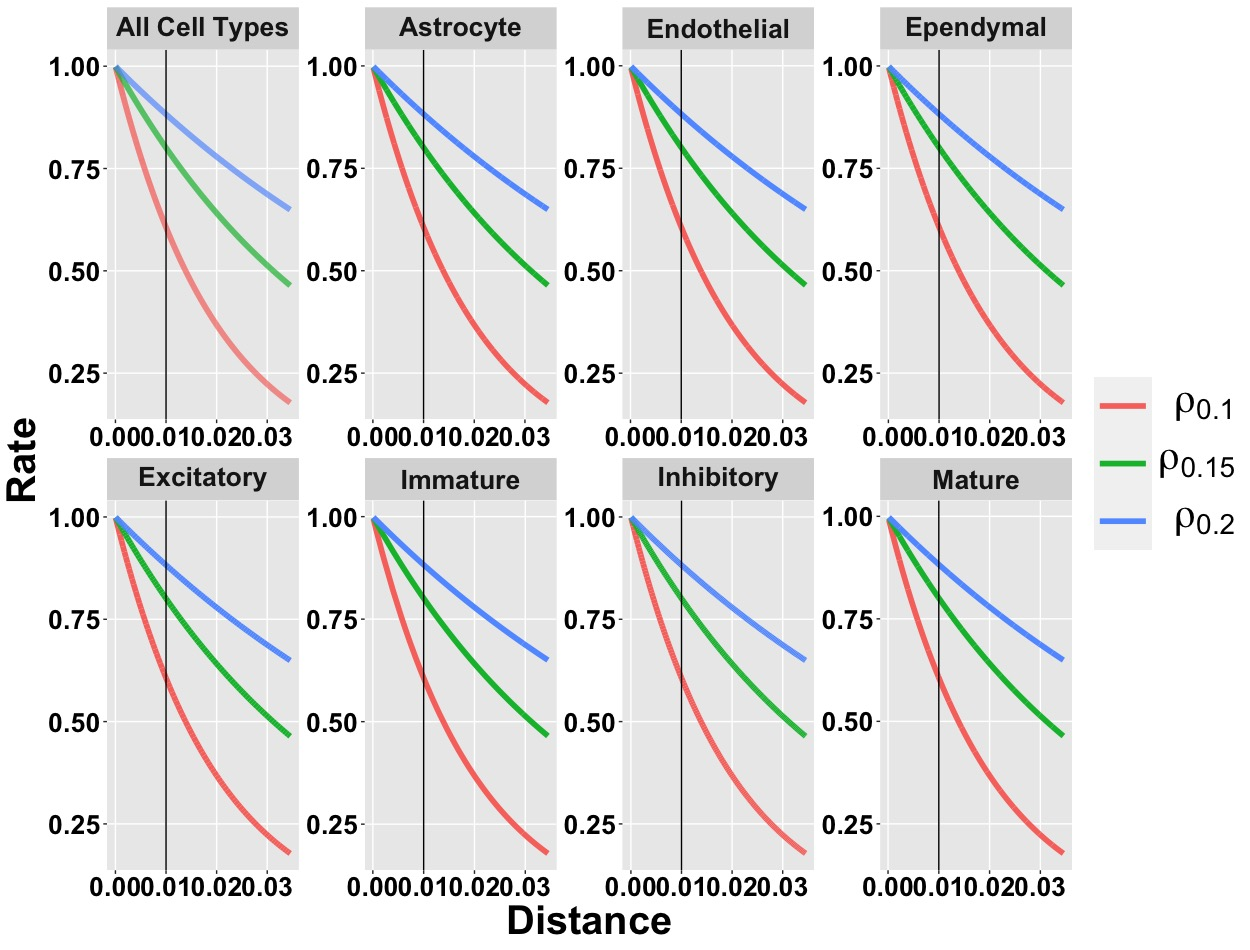
\includegraphics[width=0.8\linewidth]{images/Merfish_induced_correlation_final} 

}

\caption{Induced correlation plot for the Merfish data}\label{fig:induceCORR}
\end{figure}

\hypertarget{comparative-analysis-with-different-norm-measures}{%
\section{Comparative analysis with different norm measures}\label{comparative-analysis-with-different-norm-measures}}

We consider the simulation setting discussed in the section 3 of the manuscript. The \(5\) different methods are compared w.r.t. different norms other than \textbf{RV coefficent} \citep{robert1976unifying}. The \textbf{RV coefficent} between two matrices \(S_{1}\) and \(S_{2}\) is defined as \[\text{RV}(S_{1},S_{2}) = \frac{ tr(  S_{1}^{T} S_{2} ) }{ \sqrt{ tr(  S_{1}^{T} S_{1} )  tr(  S_{2}^{T} S_{2} ) }  }.\] We consider 4 different norms:

I. \textbf{Euclidean or Frobenius}
\[
d_{E}(S_{1},S_{2}) = \mid \mid S_{1} - S_{2} \mid \mid, 
\]
II. \textbf{Log-Euclidean}
\[
d_{L}(S_{1},S_{2}) = \mid \mid \log(S_{1}) - \log(S_{2}) \mid \mid,
\]
III. \textbf{Root Euclidean}
\[
d_{H}(S_{1},S_{2}) = \mid \mid S_{1}^{1/2} - S_{2}^{1/2} \mid \mid, 
\]

\begin{enumerate}
\def\labelenumi{\Roman{enumi}.}
\setcounter{enumi}{3}
\tightlist
\item
  \textbf{Riemanian}
  \[
  d_{R}(S_{1},S_{2}) = \mid \mid S_{1}^{-1/2} S_{2} S_{1}^{-1/2} \mid \mid.
  \]
\end{enumerate}

Figure \ref{fig:Euclid}, \ref{fig:RootEuclid}, \ref{fig:LogEuclid} and \ref{fig:ReiEuclid} are boxplot of distances between true \((\Sigma_{True})\) and estimated \((\Sigma_{Est})\) covariance matrices where the distances are measured in Euclidean, root Euclidean, log Euclidean and Riemanian norms \citep{dryden2009non} respectively. In all the norms we observe that spatial settings are performing better in terms of estimation than the no-spatial settings. Among the spatial settings the estimation accuracy increase with an increment in induced spatial correlation.

\begin{figure}

{\centering 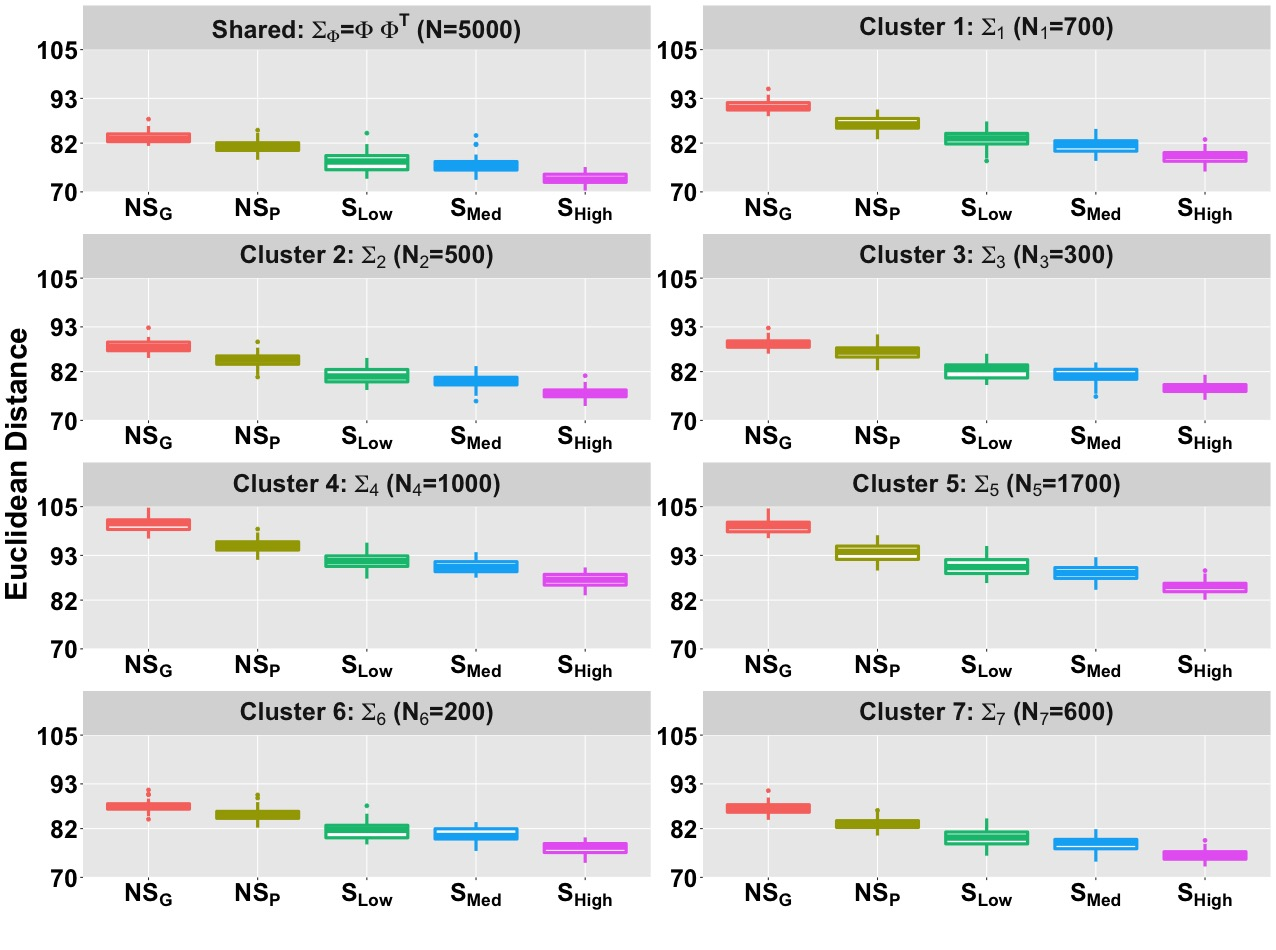
\includegraphics[width=0.8\linewidth]{images/Distance_Euclidean_plot} 

}

\caption{Boxplot of **Euclidean** distance $d_E(\Sigma_{True}, \Sigma_{Est})$ across  $50$ replicates for $\Sigma_{\Phi} = \Phi \Phi^{T}$ and $\Sigma_{l}$ $(l = 1, \dots , L)$. We compare the Euclidean distance for different method settings.}\label{fig:Euclid}
\end{figure}

\begin{figure}

{\centering 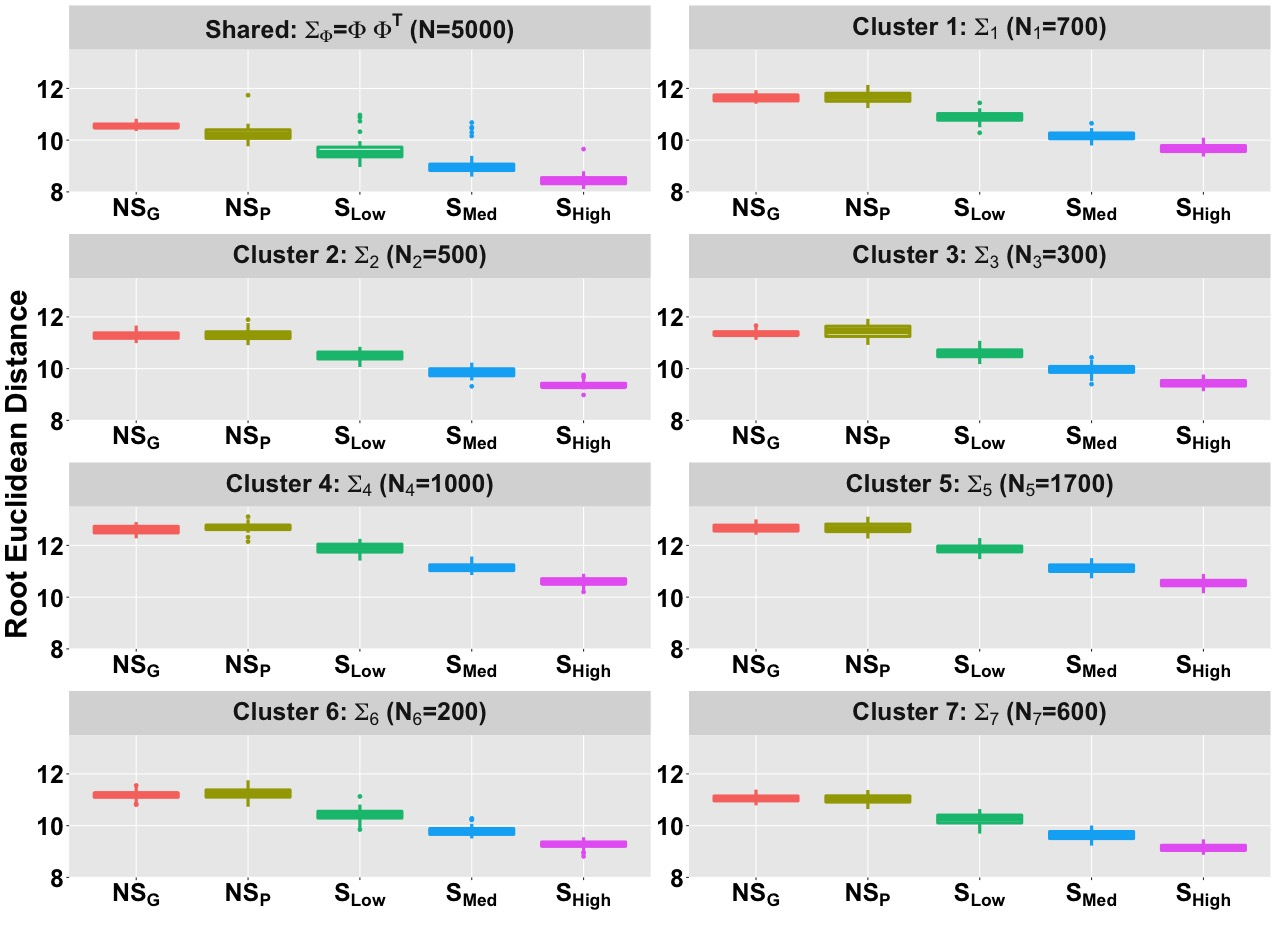
\includegraphics[width=0.8\linewidth]{images/Root_Euclidean_plot} 

}

\caption{Boxplot of **root Euclidean** distance $d_{H}(\Sigma_{True}, \Sigma_{Est})$ across  $50$ replicates for $\Sigma_{\Phi} = \Phi \Phi^{T}$ and $\Sigma_{l}$ $(l = 1, \dots , L)$. We compare the root Euclidean distance for different method settings.}\label{fig:RootEuclid}
\end{figure}

\begin{figure}

{\centering 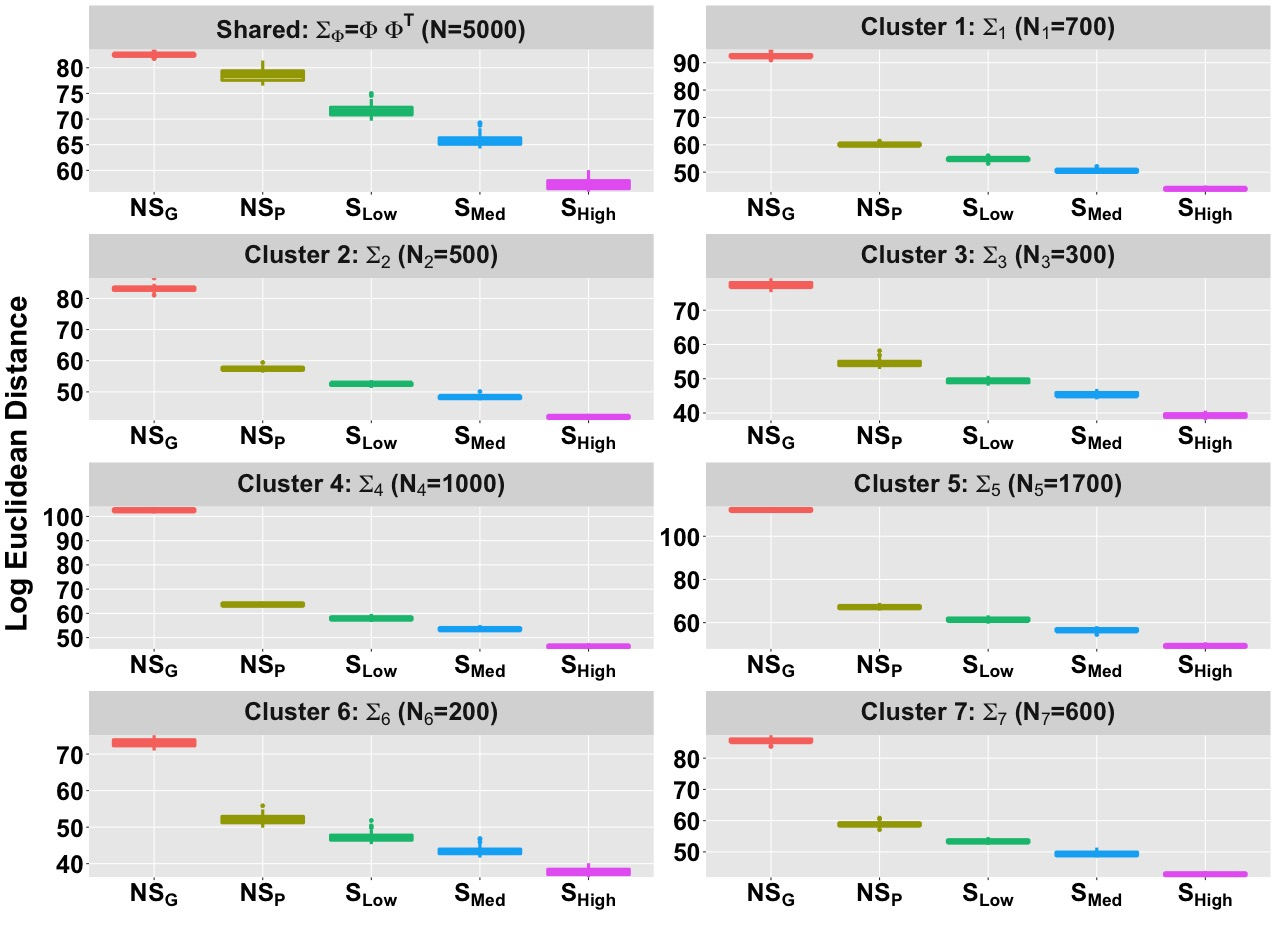
\includegraphics[width=0.8\linewidth]{images/Log_Euclidean_plot} 

}

\caption{Boxplot of **log Euclidean** distance $d_{L}( \Sigma_{True}, \Sigma_{Est})$ across  $50$ replicates for $\Sigma_{\Phi} = \Phi \Phi^{T}$ and $\Sigma_{l}$ $(l = 1, \dots , L)$. We compare the log Euclidean distance for different method settings.}\label{fig:LogEuclid}
\end{figure}

\begin{figure}

{\centering 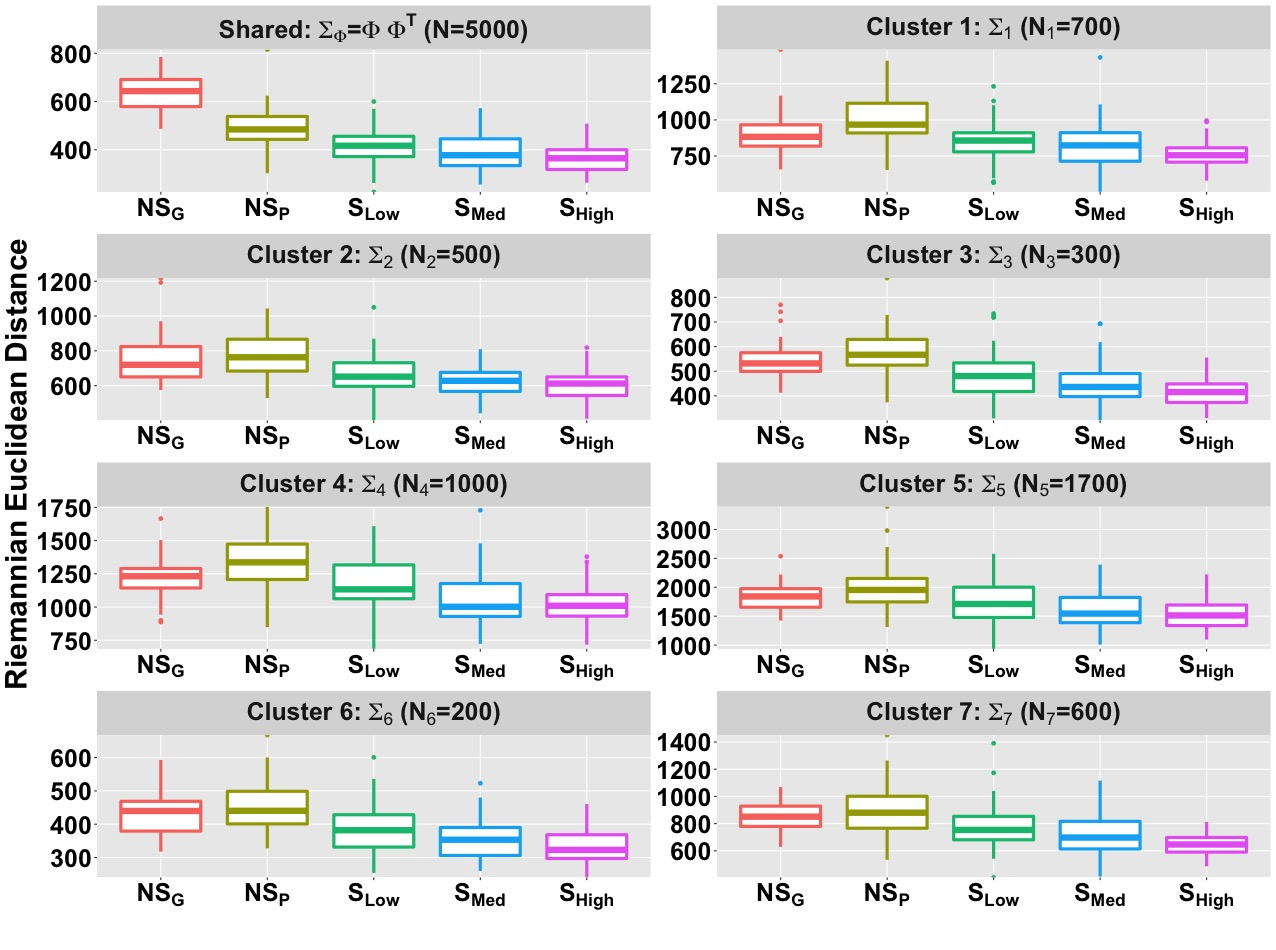
\includegraphics[width=0.8\linewidth]{images/Rei_Euclidean_plot} 

}

\caption{Boxplot of **Riemanian** distance $d_{R}( \Sigma_{True}, \Sigma_{Est})$ across  $50$ replicates for $\Sigma_{\Phi} = \Phi \Phi^{T}$ and $\Sigma_{l}$ $(l = 1, \dots , L)$. We compare the Riemanian distance for different method settings.}\label{fig:ReiEuclid}
\end{figure}

\hypertarget{estimation-of-latent-factors}{%
\section{Estimation of latent factors}\label{estimation-of-latent-factors}}

We follow same procedure from section 3.3 of \citet{de2018bayesian} to estimate shared and cluster specific number of factors i.e.~\(K\) and \(K_{c}\) \((c=1,2, \dots C)\). Figure \ref{fig:factor1} shows shared and cluster specfic estimated factor loadings accross \(50\) replicates for \(5\) different methods. Figure \ref{fig:factor2} shows the median estimate of shared and cluster specfic factor loadings for \(5\) different methods. From both figures one can observe that spatial settings are estimating the loadings more precisely than the non-spatial settings.

\begin{figure}

{\centering 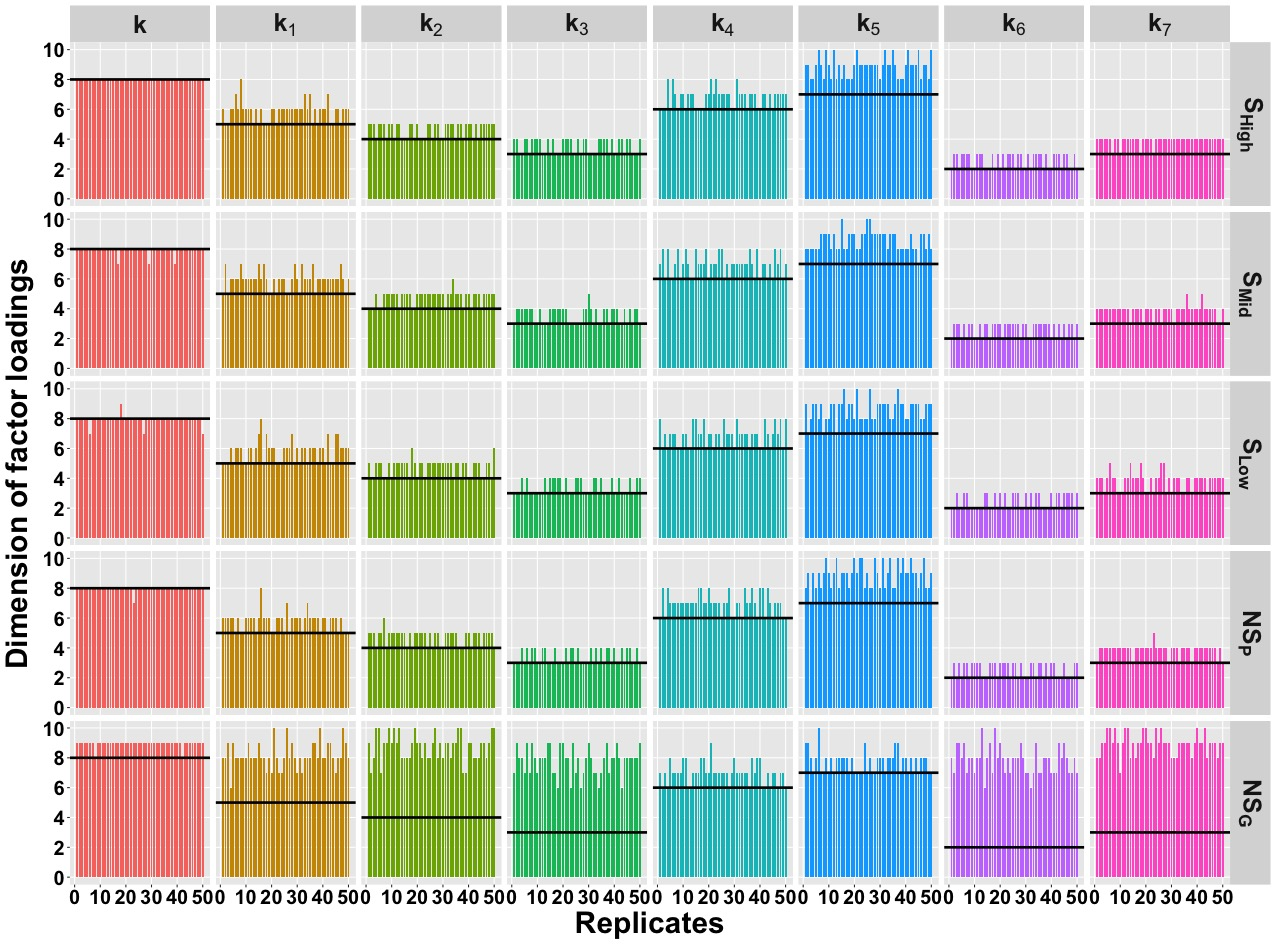
\includegraphics[width=0.8\linewidth]{images/Loading_Dimension_plot} 

}

\caption{Estimated dimension of factor loadings for shared and cluster specific cases accross $50$ replicates. Black solid line denotes the true dimensions.}\label{fig:factor1}
\end{figure}

\begin{figure}

{\centering 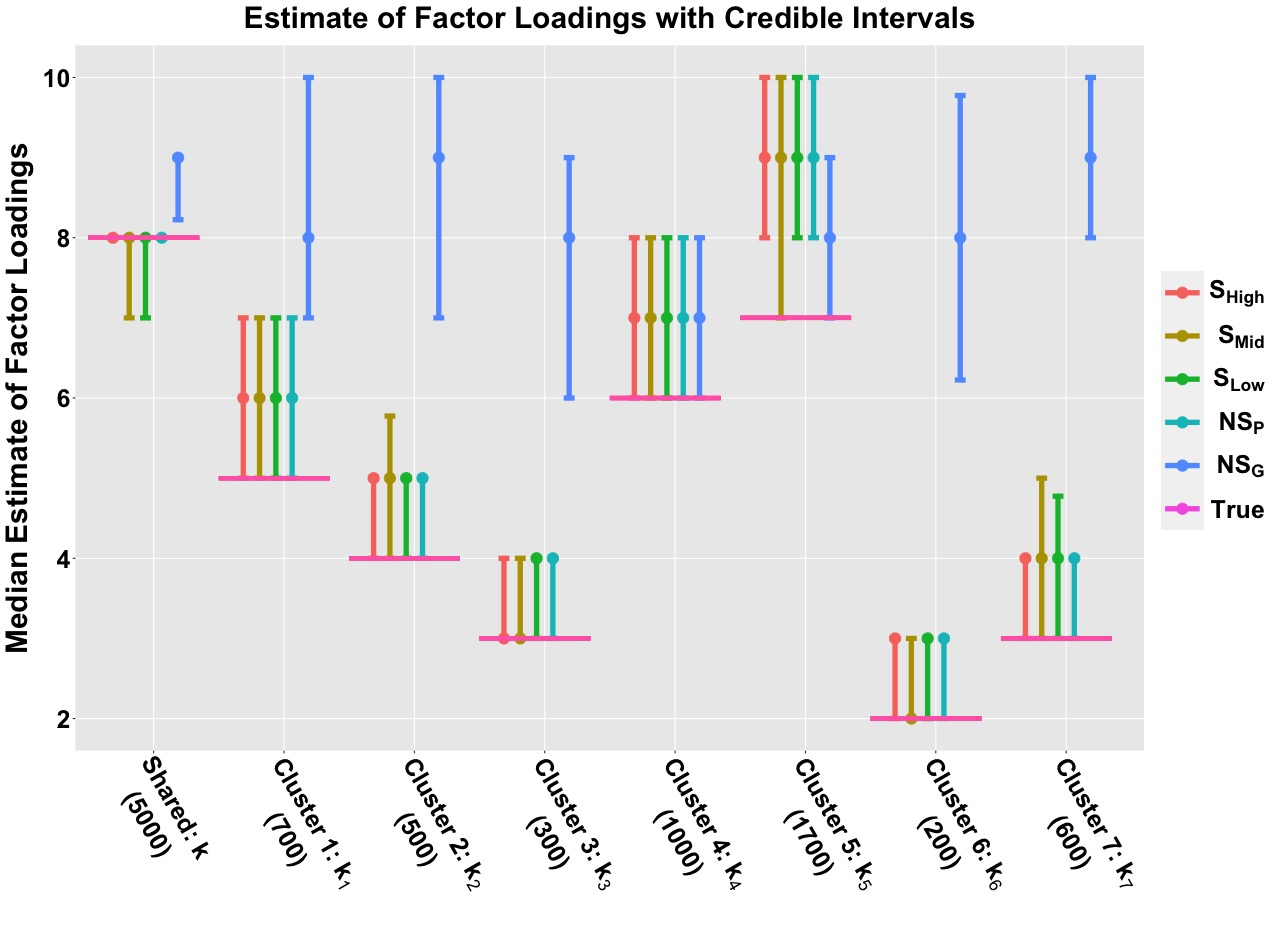
\includegraphics[width=0.8\linewidth]{images/Median_Loading_plot} 

}

\caption{Estimated Factor loadings with credible intervals.}\label{fig:factor2}
\end{figure}

\hypertarget{realdata}{%
\chapter{Real Data Analysis}\label{realdata}}

We applied the SpaceX method on two spatial transcriptomics datasets which are obtained from the preoptic region of the mouse hypothalamus \citep{Moffitteaau5324} and the human breast cancer dataset \citep{staahl2016visualization}. Here we provide details of preprocessing and exploratory analysis of both datasets in section \ref{exploratory}. We illustrate the detailed application of the community detection algorithm on those two datasets in section \ref{communitydetection}.

\hypertarget{exploratory}{%
\section{Exploratory analysis of the datasets}\label{exploratory}}

\hypertarget{merfish-data}{%
\subsection{Merfish Data}\label{merfish-data}}

The MERFISH dataset is obtained from the preoptic area of the mouse hypothalamus \citep{Moffitteaau5324}. The dataset consists of \(160\) genes and corresponding gene expressions are measured in \(4975\) spatial locations. There are \(7\) pre-determined spatial clusters in the dataset named Astrocyte, Endothelial, Ependymal, Excitatory, Inhibitory, Immature, Mature, and the corresponding sizes are \(724\), \(503\), \(314\), \(1024\), \(1694\), \(168\), \(385\) respectively. The dataset consists of \(2\) more clusters named Microglia, Pericytes with cluster sizes \(90\), \(73\) respectively which are less than \(100\). Those two clusters are removed from the dataset. After removing those two clusters, we have gene expressions from \(4812\) locations corresponding to \(160\) genes. There are no genes with more than \(95\%\) zeros reads. The left panel of Figure \ref{fig:zeroperMF} shows the violin plot of the percentage of zero reads among the genes for each cluster in the MERFISH dataset. The Umap representation of the Merfish data has been provided on the right panel of Figure \ref{fig:zeroperMF}.

\begin{figure}

{\centering \includegraphics[width=0.9\linewidth]{images/Merfish_zero_umap} 

}

\caption{Left panel shows the violin plot of percentage of zero reads among the genes for each cluster w.r.t. Merfish data and the right panel shows the Umap.}\label{fig:zeroperMF}
\end{figure}

\hypertarget{breast-cancer-data}{%
\subsection{Breast Cancer Data}\label{breast-cancer-data}}

The human breast cancer dataset contains expression levels from \(5262\) genes measured at \(250\) locations \citep{staahl2016visualization}. We use the SPARK method with \(5\%\) FDR cut-off on p-values to detect \(290\) spatially expressed genes to carry forward our analysis. The violin plot of the percentage of zero reads among the genes for each spatially contiguous cluster in the Breast cancer dataset is shown in the left panel of Figure \ref{fig:BCperzero}. On the right panel of Figure \ref{fig:BCperzero}, we have provided the Umap.

\begin{figure}

{\centering 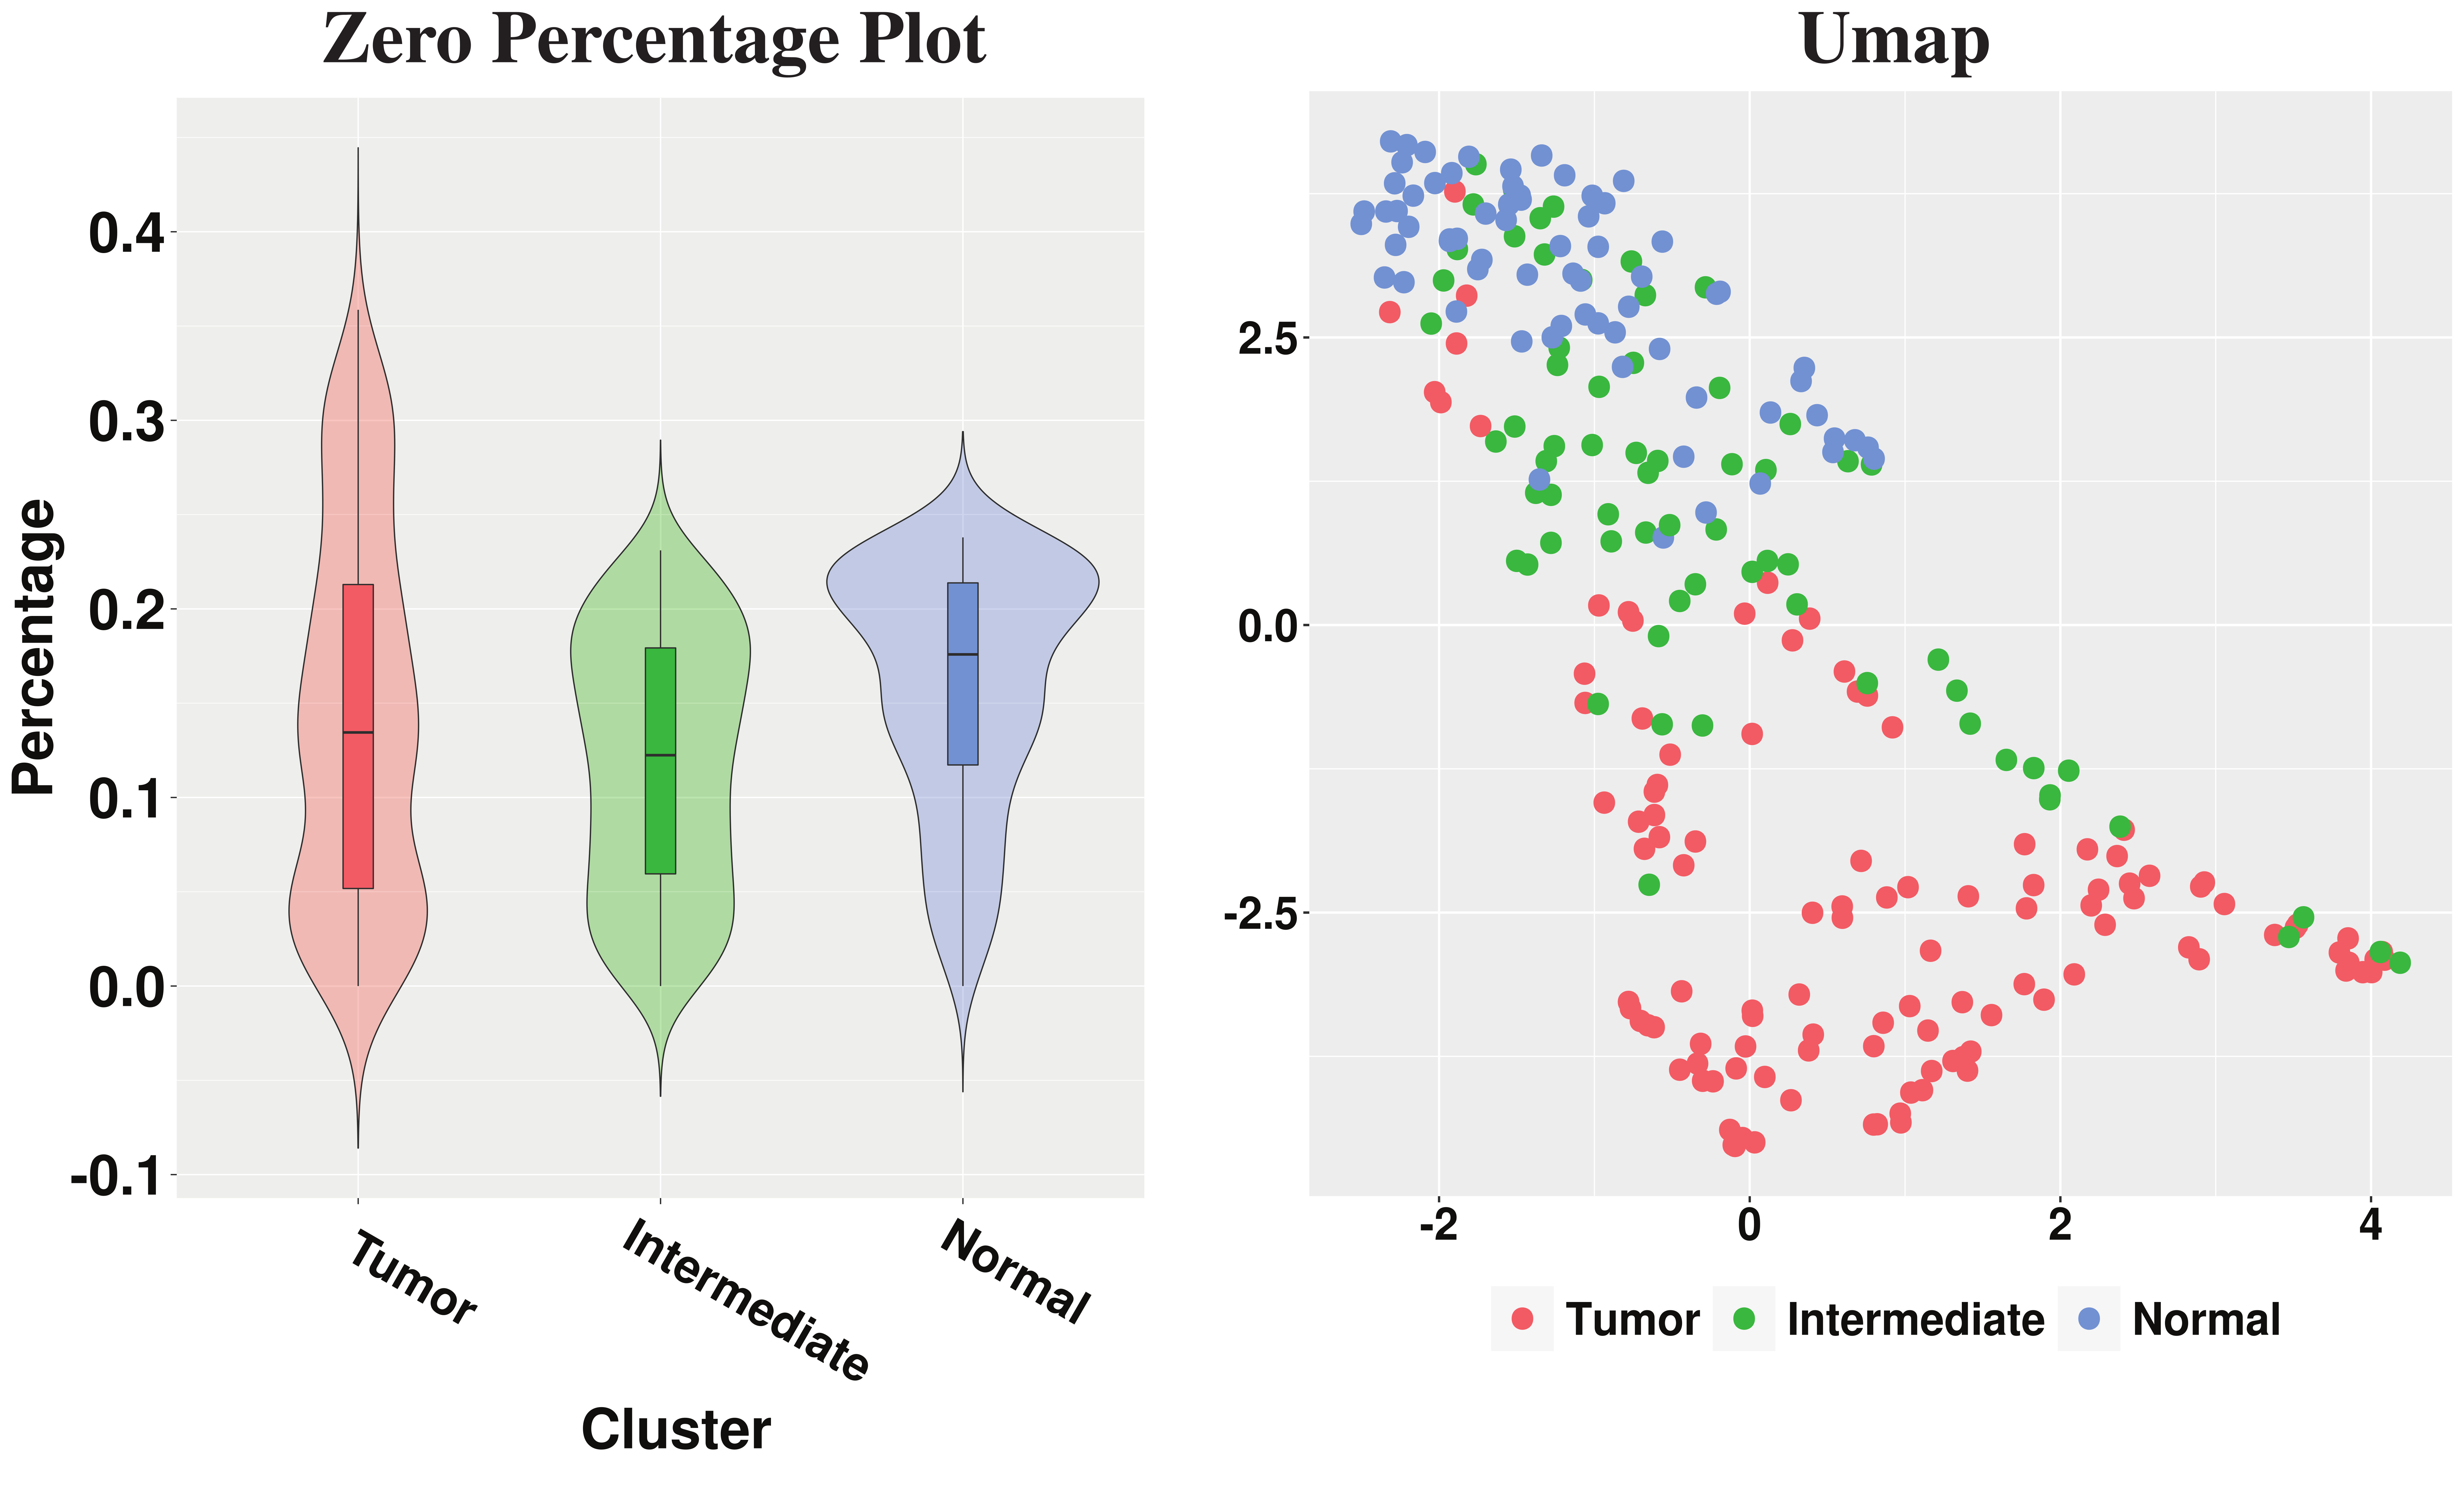
\includegraphics[width=0.8\linewidth]{images/BC_zero_umap} 

}

\caption{On the left panel, we have violin plot of percentage of zero reads among the genes for each cluster w.r.t. Breast Cancer data and the Umap is shown on the right panel.}\label{fig:BCperzero}
\end{figure}

\hypertarget{communitydetection}{%
\section{Community detection}\label{communitydetection}}

The community detection is a downstream analysis of the shared and cluster-specific networks which are obtained from the SpaceX method. The communities are detected by optimizing modularity over partitions in a network structure \citep{brandes2007modularity}. Figure \ref{fig:comMERFISH} and \ref{fig:comBC} show the detected community modules from shared and cluster-specific co-expression networks for MERFISH and breast cancer data respectively.

\begin{figure}

{\centering \includegraphics[width=0.95\linewidth]{images/merfishCom} 

}

\caption{Shared and cell-type specific community detection for Merfish data}\label{fig:comMERFISH}
\end{figure}

\begin{figure}

{\centering 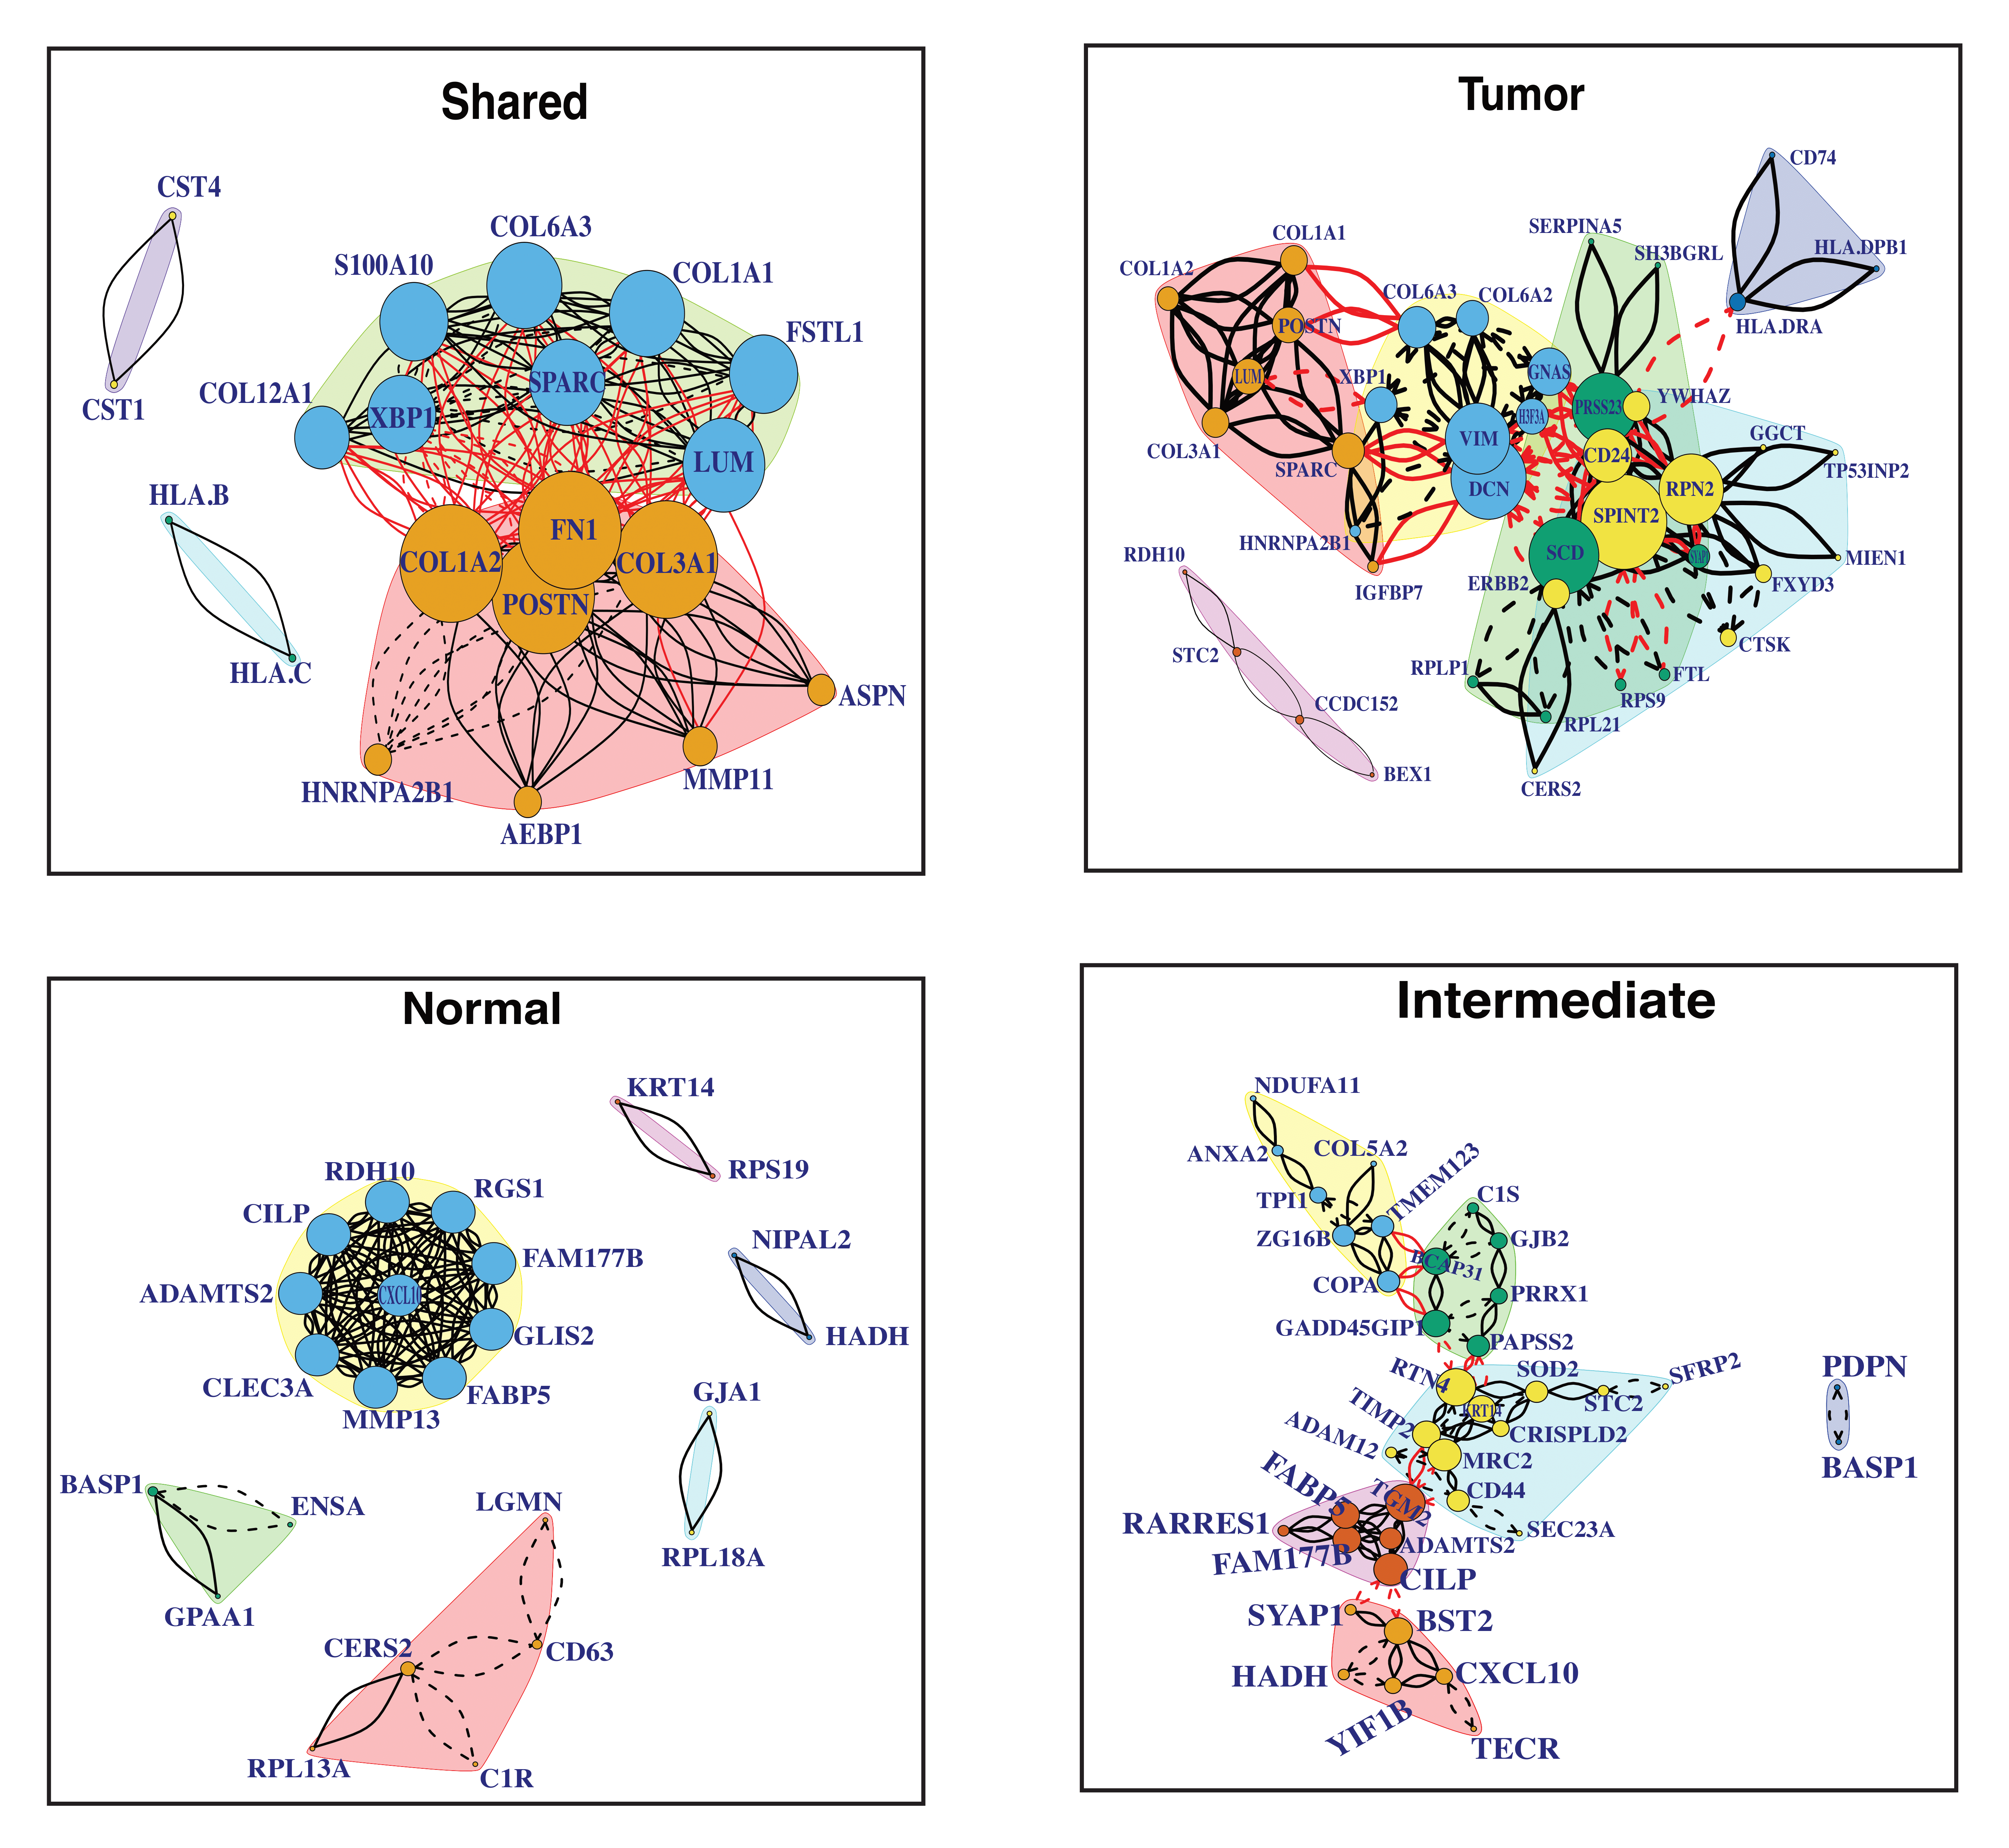
\includegraphics[width=0.8\linewidth]{images/BC_Com} 

}

\caption{Shared and cell-type specific community detection for Breast cancer data}\label{fig:comBC}
\end{figure}

\hypertarget{list-of-hub-genes-and-edges}{%
\section{List of hub genes and edges}\label{list-of-hub-genes-and-edges}}

A detailed list of hub genes and top edges for both the datasets can be found at \url{https://github.com/SatwikAch/SpaceX}.

\hypertarget{ImplementSpaceX}{%
\chapter{Implementation of SpaceX}\label{ImplementSpaceX}}

SpaceX function extimates shared and cluster specfic gene co-expression networks for spatial transcriptomics data. More details about the SpaceX method can be found in the main manuscript. See below for detailed discussion on installation of SpaceX package, Data inputs and outputs followed by an example.

\hypertarget{installation}{%
\section{Installation}\label{installation}}

You can install the released version of SpaceX from (\url{https://github.com/SatwikAch/SpaceX}) with:

\begin{Shaded}
\begin{Highlighting}[]
\NormalTok{devtools}\SpecialCharTok{::}\FunctionTok{install\_github}\NormalTok{(}\StringTok{"SatwikAch/SpaceX"}\NormalTok{)}
\FunctionTok{library}\NormalTok{(SpaceX)}
\end{Highlighting}
\end{Shaded}

\hypertarget{data-inputs}{%
\section{Data inputs}\label{data-inputs}}

Please make sure to provide both inputs as dataframe.

The first input is \textbf{Gene\_expression\_mat} which is \(N \times G\) dataframe. Here \(N\) denotes the number of spatial locations and \(G\) denotes number of genes.

The second input is \textbf{Spatial\_locations} is a dataframe which contains spatial coordinates.

The third input is \textbf{Cluster\_annotations}.

\hypertarget{output}{%
\section{Output}\label{output}}

You will obtain a list of objects as output.

\textbf{SigmaPhi} denotes the Shared Covariance matrix i.e.~\(\Sigma_{\Phi} = \Phi \Phi^{T}\).

\textbf{SigmaLambda} denotes the cluster specific Covaraince matrices i.e.~\(\Sigma_{\Psi^{c}} = \Psi^{c} {\Psi^{c}}^{T}\).

\hypertarget{example}{%
\section{Example}\label{example}}

Here we provide an example to run the SpaceX method.

\begin{Shaded}
\begin{Highlighting}[]
\CommentTok{\# Reading the Breast cancer data}

\CommentTok{\# Spatial locations}
\FunctionTok{head}\NormalTok{(BC\_loc)}

\CommentTok{\# Gene expression for data}
\FunctionTok{head}\NormalTok{(BC\_count) }

\CommentTok{\# Data processing}
\NormalTok{G }\OtherTok{\textless{}{-}}\FunctionTok{dim}\NormalTok{(BC\_count)[}\DecValTok{2}\NormalTok{] }\CommentTok{\# number of genes}
\NormalTok{N }\OtherTok{\textless{}{-}}\FunctionTok{dim}\NormalTok{(BC\_count)[}\DecValTok{1}\NormalTok{] }\CommentTok{\# number of locations}
\end{Highlighting}
\end{Shaded}

Next, we'll apply the SpaceX method on the Breast cancer dataset.

\begin{Shaded}
\begin{Highlighting}[]
\CommentTok{\# Application to SpaceX method}
\NormalTok{BC\_fit }\OtherTok{\textless{}{-}} \FunctionTok{SpaceX}\NormalTok{(BC\_count,BC\_loc[,}\DecValTok{1}\SpecialCharTok{:}\DecValTok{2}\NormalTok{],BC\_loc[,}\DecValTok{3}\NormalTok{])}

\CommentTok{\# SigmaPhi :: Shared Covariance matrix}
\CommentTok{\# SigmaLambda :: Cluster specific Covaraince matrices}
\end{Highlighting}
\end{Shaded}


  \bibliography{book.bib,packages.bib}

\end{document}
